\chapter{Part 2}
%Learning Objectives
%• Embedded control system design using industrial tools
%• Familiarising with a state-of-the-art timing analysis tool from
%INCHRON*
%• INCHRON is a German automotive company which has
%several well-known analysis tools used by companies like
%BMW, AUDI, Daimler etc.


\section{Introduction}
%• Very brief introduction of the overall problem setting (< page
%max)

\section{Response Time analysis}

\subsection{Response time analysis per processing unit}
%• Response time analysis per processing unit (plots and brief description)

% Table generated by Excel2LaTeX from sheet 'Sheet1'
\begin{table}[htbp]
	\centering
	\caption{By running the Matlab script ResponsetimeAnylsis\_FPP.m with the different parameters given for PU1 and PU2 these response times are obtained. These files are then delivered as PU1.m PU2.m}
	\begin{tabular}{rrrrr}
		& & & & \\
		\toprule
		PU1     & $T_1$    & $T_2$    & $T_3$    & $T_4$  $(T_s)$ \\
		\midrule
		Matlab (ms)      & 0.1     & 2.1     & 4.1     & 7.2 \\
		Inchron (ms)	& 0.1     & 2.1     & 4.1     & 7.2 \\
		
		& & & & \\
		\toprule
		PU2     & $T_5$    & $T_6$    & $T_7$    & $T_8$ \\
		\midrule
		Matlab (ms)      & 6       & 3       & 9       & 5 \\
		Inchron (ms)	 & 6       & 3       & 9       & 5 \\
		
	\end{tabular}%
	\label{tab:addlabel}%
\end{table}%


\begin{figure}[h]
	\begin{center}
		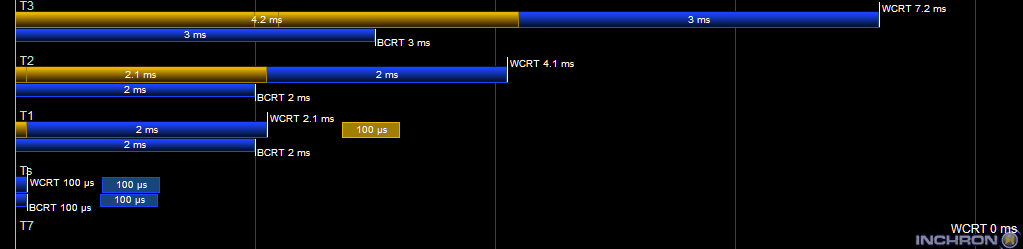
\includegraphics[width=0.7\linewidth]{img/pu1-response-time}
		\caption{}
		\label{fig:pu1rt}
	\end{center}
\end{figure}

\begin{figure}[h]
	\begin{center}
		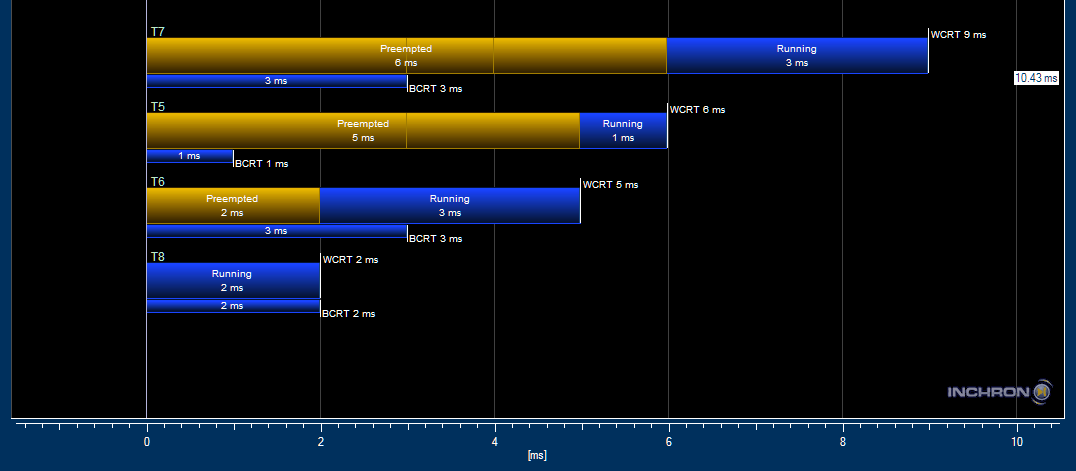
\includegraphics[width=0.7\linewidth]{img/pu2-response-time}
		\caption{}
		\label{fig:pu2rt}
	\end{center}
\end{figure}


\subsection{ Response time analysis for the CAN bus messages}
%• Response time analysis for the CAN bus messages

\section{Optimisation for sensor-to-actuator delay}
%• Optimisation for sensor-to-actuator delay (include troubleshooting)

\section{System model}
%• System model derivation, design space exploration and controller
%parameter design

\section{Design decision}
%• Your design decision and justification.

\section{Results}
%• Results
%− Response time analysis

Firstly: Response time analysis\\
Secondly: Plots from chronVIEW (before and after optimization)\\
Last: Control system input and output

\section{Conclusions}